\documentclass[float=false, crop=true]{standalone}

\usepackage{graphicx} % Required for inserting images
\usepackage{tikz}
\usepackage{xcolor}
\usepackage{pgfplots}
\usepackage{svg}
\usepackage{tikz}

\usetikzlibrary{shapes.geometric,fit,positioning,arrows.meta,calc}

\pgfplotsset{compat=1.16}

\definecolor{myGreen}{HTML}{009E73}
\definecolor{uniBlue}{HTML}{00467f}

\begin{document}

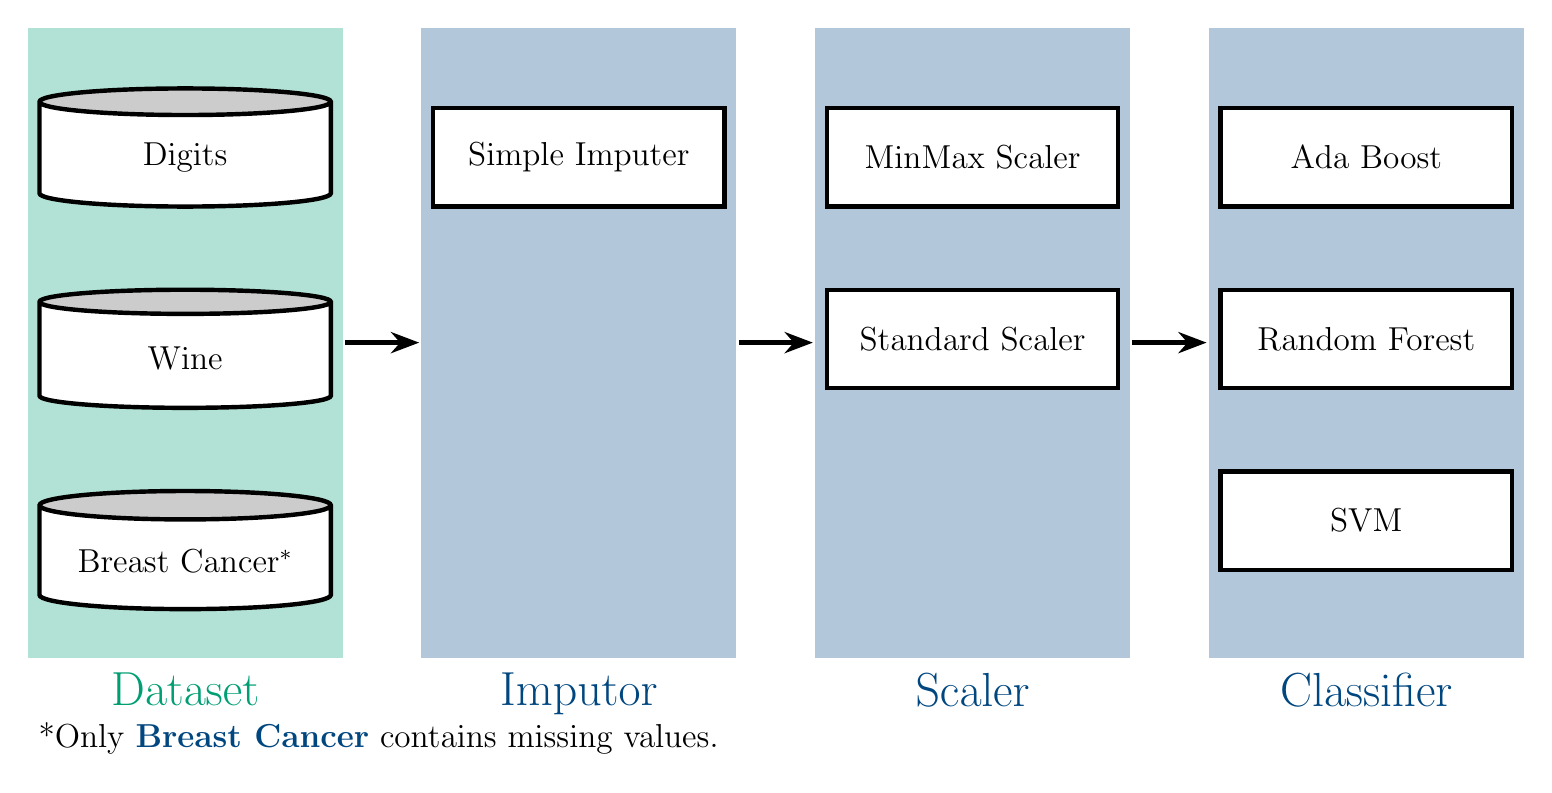
\begin{tikzpicture}[ultra thick]
    \large

    % Shapes
    \tikzstyle{block}=[rectangle, minimum height=8cm, minimum width=4cm]
    \tikzstyle{data}=[
        cylinder, 
        draw,
        cylinder uses custom fill, 
        cylinder body fill = white, 
        cylinder end fill = gray!40,
        shape border rotate=90, 
        aspect=.25, 
        align=center, 
        minimum width=3.7cm, 
        minimum height=1.5cm]
    \tikzstyle{model}=[rectangle, draw, fill=white, minimum width=3.7cm, minimum height=1.25cm, align=center]

    % Blocks
    \node[block, fill=myGreen!30, label={[align=center]below:\LARGE \textcolor{myGreen}{Dataset}}] at (2,4) (blockData) {};
    \node[block, fill=uniBlue!30, label={[align=center]below:\LARGE \textcolor{uniBlue}{Imputor}}] at (2+5,4) (blockPre1) {};
    \node[block, fill=uniBlue!30, label={[align=center]below:\LARGE \textcolor{uniBlue}{Scaler}}] at (2+5*2,4) (blockPre2) {};
    \node[block, fill=uniBlue!30, label={[align=center]below:\LARGE \textcolor{uniBlue}{Classifier}}] at (2+5*3,4) (blockClf) {};

    % Arrows
    \draw[-Stealth] (blockData) -- (blockPre1);
    \draw[-Stealth] (blockPre1) -- (blockPre2);
    \draw[-Stealth] (blockPre2) -- (blockClf);

    % Datasets
    \node[data, above=1.7cm of blockData.center] (data1) {Digits};
    \node[data, below=of data1.south] (data2) {Wine};
    \node[data, below=of data2.south, aspect=.12] (data3) {Breast Cancer$^*$};

    % Preprocessing 1
    \node[model, above=1.7cm of blockPre1.center] (p1) {Simple Imputer};

    % Preprocessing 2
    \node[model, above=1.7cm of blockPre2.center] (p2Minmax) {MinMax Scaler};
    \node[model, below=of p2Minmax.south] (p2Std) {Standard Scaler};

    % Classifier
    \node[model, above=1.7cm of blockClf.center] (clf1) {Ada Boost};
    \node[model, below=of clf1.south] (clf2) {Random Forest};
    \node[model, below=of clf2.south] (clf3) {SVM};

    \node[below=of blockData.south west, anchor=west] {*Only \textbf{\textcolor{uniBlue}{Breast Cancer}} contains missing values.};
    
    % Mash
    % \draw[lightgray, step=1, ultra thin] (0,0) grid (19,8);
\end{tikzpicture}
 
\end{document}
